%----------------------------------------------------------------------------------------------------
\chapter{SVN}
%----------------------------------------------------------------------------------------------------
%
SVN is the name of the software we use to control the source of \telemacsystem. The
link \url{http://en.wikipedia.org/wiki/Version_control} will give you an
explanation of what a source control is.
The section below will give you a guide on how to perform a few actions
using SVN.
%
\begin{figure}[H]
    \centering
    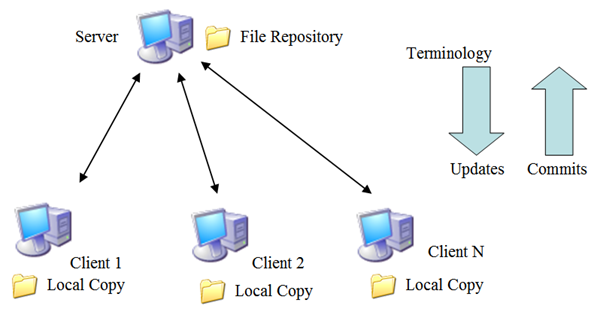
\includegraphics[scale=0.6]{graphics/svn-image.png}
    \caption{SVN structure}
    \label{fig:svn-struct}
\end{figure}
If you are not into command line a few software give you a graphical interface
to handle your repository: kdeSVN, RapidSVN...
%
%
%----------------------------------------------------------------------------------------------------
\section{Create a work copy}
%----------------------------------------------------------------------------------------------------
%
%
\begin{lstlisting}[language=bash]
svn checkout http://svn.opentelemac.org/svn/opentelemac/trunk DEST
\end{lstlisting}
Create a local repository in $DEST$ of the subversion server on the computer.
If you want a working copy of your branch just replace
\url{http://svn.opentelemac.org/svn/opentelemac/trunk} by
\url{http://svn.opentelemac.org/svn/opentelemac/branches/branchname} where
$branchname$ is the name of your branch.\\
%
\begin{WarningBlock}{Warning:}
If your are using a network proxy you need to modify the \verb"$HOME/.subversion/server"
file by adding the following lines under the line \verb"[global]":
\begin{lstlisting}[language=bash]
[global]
...
http-proxy-host = proxypac.edf.fr
http-proxy-port = 3128
http-proxy-username = NNI
http-proxy-password = SesamePassword
...
\end{lstlisting}
Where:
\begin{itemize}
\item \textbf{http-proxy-host} is the address of your proxy.
\item \textbf{http-proxy-port} is the port of your proxy.
\item \textbf{http-proxy-username} is the login for your proxy.
\item \textbf{http-proxy-password} is the password for your proxy.
\end{itemize}
\end{WarningBlock}
%
%
%----------------------------------------------------------------------------------------------------
\section{SVN commands}
%----------------------------------------------------------------------------------------------------
%
%
Here is a list of a few useful SVN commands:
%
\begin{lstlisting}[language=bash]
svn help [command]
\end{lstlisting}
You can get a detailed description of any command.
%
%
\begin{lstlisting}[language=bash]
svn update
\end{lstlisting}
Update your local repository with the server repository. This will add all the
modification made on the subversion server on your local repository.
%
\begin{lstlisting}[language=bash]
svn commit -m "Message about what the commit contains"
\end{lstlisting}
Push your local modifications on the server repository. This will add all the
modifications you made on your local repository on the server repository. You
should alway do an update before doing a commit in case someone else did some
modifications before you. Anyway if you are not up to date SVN will not allow
the commit. The $-m$ option allows you to write directly the message associated
with the commit instead of having a text editor opening. Those messages should
summarize what the commit is adding.\\
The message should respect the following template "[\textit{Type}]
\textit{Text}" where:
\begin{itemize}
\item If you have a cue ticket associated to the commit:
\begin{itemize}
\item Type = "fix \#\textit{id}" ,"feature \#id" or "vnv \#id" where id is the id of
the cue ticket
\item Text = Title of the cue ticket
\end{itemize}
\item Otherwise:
\begin{itemize}
\item Type = doc : If ti concerns the documentation
\item Type = scripts : If it concerns the scripts of the system
\item Type = src : General action on the source code (code convention, trimming removing white spaces...)
\item Type = vnv : Verification \& Validation
\item Text = Description of the commit
\end{itemize}
\end{itemize}
If the commit contains more than one action repeat the process on a new line.
%
\begin{lstlisting}[language=bash]
svn log
\end{lstlisting}
Display all the commit messages.
\\
\begin{CommentBlock}{Tips:}
If the output is too big use the following command instead and press q to exit.
\begin{lstlisting}[language=bash]
svn log|less
\end{lstlisting}
\end{CommentBlock}
%
\begin{lstlisting}[language=bash]
svn status
\end{lstlisting}
Display the status on all the file in the local repository. If a file is
modified, added, missing or deleted. See "svn help status" for more
information.
%
\begin{lstlisting}[language=bash]
svn add/delete/move
\end{lstlisting}
Add/Delete/Move a folder/file to the SVN repository.
%
\begin{lstlisting}[language=bash]
svn info
\end{lstlisting}
Display information about the local repository. Like the address of the server
repository, the last revision, \ldots
%
\begin{lstlisting}[language=bash]
svn revert FILE
\end{lstlisting}
Cancel the local modifications on the file $FILE$. This cannot be undone so
tread lightly with this command.
%
%----------------------------------------------------------------------------------------------------
\section{Update your branch with the latest version of the trunk}
%----------------------------------------------------------------------------------------------------
%
One of the conditions for validating a development is that it is up to date
with the trunk.  In order to ease that step that can be some times painful it
is recommended to do that action weekly.  This way you do smaller updates
instead of a massive one.
\paragraph{The commands}
\begin{enumerate}
\item Go into the branch main folder.
\begin{lstlisting}[language=bash]
cd mybranch
\end{lstlisting}
Where $mybranch$ is the path to your local checkout of your branch.
\item Launch the merge command with $rev$ being the last revision of the trunk
you are up to date with. If this is the first time you are updating it is the
revision at which your branch was created (can be found in the log given by the
"svn log" command) otherwise you can get that value using the following
command:
\begin{lstlisting}[language=bash]
svn propget svn:mergeinfo .
\end{lstlisting}
It should return something like that:
\begin{lstlisting}[language=bash]
/branches/guppy:187-256,4145-4591
/branches/jewelpuffer:4665-4793
/branches/rainbowfish:2559-2958,4070-4614,4623-4798
/branches/salmon:138-254,272-286
/trunk:541-3423,4222-4817
\end{lstlisting}
The value you want is in the line \verb+/trunk:541-3423,4222-4817+. You need
the last digits i.e. $4817$.  Then you replace in the following command rev by
that number.
\begin{lstlisting}[language=bash]
svn merge -r rev:HEAD http://svn.opentelemac.org/svn/opentelemac/trunk .
\end{lstlisting}
The $HEAD$ value will be automatically replaced by the latest revision of the
trunk.
\item If the merge generates any conflict you will need to resolve them (See
Section \ref{conflict}).
\item When everything is resolved. You need to commit the merged version. Add
the trunk revision number to the commit message for information.
\begin{lstlisting}[language=bash]
svn commit -m "Merged with revision rev of the trunk"
\end{lstlisting}
\end{enumerate}
%
\paragraph{Conflicts}
\label{conflict}
When using SVN you sometime encounter a conflict. For example if two persons
are working on the same file. You will get the following message:
\begin{lstlisting}[language=bash]
conflict discovered in 'foo.c'.
Select: (p) postpone, (df) diff-full, (e) edit,
        (mc) mine-conflict, (tc) theirs-conflict,
        (s) show all options:
\end{lstlisting}
Here is a listing of all the options available:
\begin{lstlisting}[language=bash]
(e)  edit             - change merged file in an editor
(df) diff-full        - show all changes made to merged file
(r)  resolved         - accept merged version of file

(dc) display-conflict - show all conflicts (ignoring merged version)
(mc) mine-conflict    - accept my version for all conflicts (same)
(tc) theirs-conflict  - accept their version for all conflicts (same)

(mf) mine-full        - accept my version of entire file (even non-conflicts)
(tf) theirs-full      - accept their version of entire file (same)

(p)  postpone         - mark the conflict to be resolved later
(l)  launch           - launch external tool to resolve conflict
(s)  show all         - show this list
\end{lstlisting}
%
If you do not know what to do select option $p$. This option will generate the
following files near the one in conflict:
\begin{itemize}
\item $foo.c.mine$ which contains your local version of the file
\item $foo.c.r44$ which contains the file at the last revision on the server
repository.
\item $foo.c$ which contains both of the previous files with the following
syntax:
\end{itemize}
\begin{lstlisting}[language=bash]
<<<<<<< .mine
This is fun stuff!
=======
This is a documentation file
>>>>>>> .r6
\end{lstlisting}
You need to select in the file what part should be kept. Once the file is
correct to resolve the conflict launch the following command:
\begin{lstlisting}[language=bash]
svn resolved foo.c
\end{lstlisting}
\begin{WarningBlock}{Warning:}
"svn resolved" tells SVN that you solved the conflict and that is all. So
thread lightly with that option if you call "svn resolved" on a file in which you
did not made the modifications it will most likely break the compilation as the
"\verb!<<<<!" will still be in the file.\\
\end{WarningBlock}
\\
%
\begin{CommentBlock}{Tips:}
You can add the option "--accept ARG" to the merge command to give an automatic
response in case of a conflict.
\begin{lstlisting}[language=bash]
 --accept ARG             : Specify the action to apply in case of conflicts
   ('postpone', 'base', 'mine-conflict', 'theirs-conflict',
    'mine-full', 'theirs-full', 'edit', 'launch')
\end{lstlisting}
\end{CommentBlock}
%
%----------------------------------------------------------------------------------------------------
\section{Merge a development into the trunk}
%----------------------------------------------------------------------------------------------------
%
The person in charge of the integration will have to follow those steps:
\begin{enumerate}
\item Go into the trunk main folder.
\begin{lstlisting}[language=bash]
cd mytrunk
\end{lstlisting}
Where \textit{mytrunk} is a SVN repository pointing on the trunk. The trunk
repository should be clean of every modification to be even more prepared, the
command "svn status" should return nothing.
\item Launch the merge command with $rev1$ being the revision at which the
development associated with the merge started. The $rev2$ value will be
automatically replaced by the latest revision of the branch.
\begin{lstlisting}[language=bash]
svn merge -r rev1:rev2 --reintegrate http://svn.opentelemac.org/svn/opentelemac/branches/mybranch .
\end{lstlisting}
\item If the merge generates any conflict you will need to resolve them (See
Section \ref{conflict}).
\item The "--reintegrate" option will tell svn to bypass the commit that were
merged from the trunk, i.e it will only merge the developments.
\item When everything is okay. You must now commit the merged version. Add the
trunk revision number to the commit message for information.
\begin{lstlisting}[language=bash]
svn commit -m "Merged of branch mybranch for feature #??? of the cue"
\end{lstlisting}
\end{enumerate}
%
%----------------------------------------------------------------------------------------------------
\section{Fresh start on branch}
%----------------------------------------------------------------------------------------------------
%
You have just finished your development and want to get ready for the next one?
%
To do that efficiently use the following script:
\begin{lstlisting}[language=bash]
#!/bin/bash
if [[ $# -ne 3 ]];then
  echo 'Usage: freshstart.sh branch-name path-to-branch revision-of-trunk'
  echo 'Usage: freshstart.sh rainbowfish ~/opentelemac/branches/rainbowfish 6666'
  exit 1
fi
branchname=$1
mybranch=$2
rev=$3
delaysvn=/projets/projets.002/systel.002/bin/delaysvn.sh
# Moving into the branch folder
cd $mybranch
# Removing all local modifications execpt in the "configs" and "builds"folder
svn stat|grep -i ? |grep -vi configs/|grep -vi builds|sed -e "s/^?[ ]*//g"|tr '\n' ' '|xargs rm -rvf
# Copying all the stuff from the latest revision of the trunk to the branch
~/bin/delaysvn.sh svn export --force http://svn.opentelemac.org/svn/opentelemac/trunk .
# Adding new files
svn stat|grep -i ? |grep -vi configs/|grep -vi builds|sed -e "s/^?[ ]*//g"|tr '\n' ' '|xargs svn add
# Removing file if necessary
# Running diff between trunk and branch
$delaysvn svn diff http://svn.opentelemac.org/svn/opentelemac/branches/$branchname http://svn.opentelemac.org/svn/opentelemac/trunk --summarize|tee diff.log
# Getting the file to delete
grep ^D diff.log |sed -e "s|^D[ ]*http://svn.opentelemac.org/svn/opentelemac/branches/${branchname}/||g"|tr '\n' ' '| xargs svn rm
rm diff.log
# Committing the fresh version
$delaysvn svn commit -m "Fresh_start_from_r$rev"
\end{lstlisting}
And run the following command:
\begin{lstlisting}[language=bash]
freshstart.sh branch-name path-to-branch revision-of-trunk
\end{lstlisting}
Where:
\begin{itemize}
\item $branch-name$ is the name of your branch
\item $path-to-branch$ is the path on your computer to your branch
\item $revision-of-trunk$ is the revision of the trunk from which you want a
fesh start (This is just used as information for the commit message the
revision it is going to use is the latest one)
\end{itemize}
%
\begin{WarningBlock}{Warning:}
This process will completely erase any modifications you have locally on your
repository. The "svn export" command will overwrite your local files with the
latest version of the trunk.
\end{WarningBlock}
\\
Copy the text in a file and run \verb!bash file! with $file$ the name of your
file. Replace $rev$ by the revision of the trunk.
%
%----------------------------------------------------------------------------------------------------
\section{How to generate the list of your modifications}
%----------------------------------------------------------------------------------------------------
%
\label{diff}
In this part we will explain how to generate a list of the difference between
your branch and the trunk. This list id one of the item necessary to validate
your development.
\begin{lstlisting}[language=bash]
svn diff --summarize http://svn.opentelemac.org/svn/opentelemac/trunk http://svn.opentelemac.org/svn/opentelemac/branches/mybranches | tee work.diff
\end{lstlisting}
This command will write the difference into the file "work.diff" and on the
standard ouput (i.e. in the terminal).
%
